\subsection{OpenCerts}
OpenCerts  es una aplicación que permite a las entidades como escuelas, universidades, gestionen los certificados de sus alumnos
de manera segura y sin intermediarios utilizado la tecnología  Blockchain.
La aplicación no almacena los datos privados de los alumnos, sino que utilizan las claves públicas referenciadas a los usuarios. La función de las organizaciones o entidades es gestionar los certificados de los alumnos 
asociándolos a su clave pública. Los estudiantes pueden consultar, descargar y compartir 
sus certificados. El administrador valida que las entidades dadas de alta sean correctas \cite[]{opencerts_gestion_nodate}.

Funciona generando 
un código único a partir del certificado e información extra considerada como necesaria para validar el documento en el futuro, y luego se crea 
un archivo con extensión  “.opencerts”;
dicho archivo se carga al sitio web de OpenCerts y compara el contenido con el almacenado en la  Blockchain para verificar si existió el 
certificado en cuestión.
Para dar de alta los certificados usan el smart contract donde también crean los métodos para emitir o revocar un documento \cite[]{opencerts_frequently_nodate}.

\begin{figure}[H]
  \centering
  {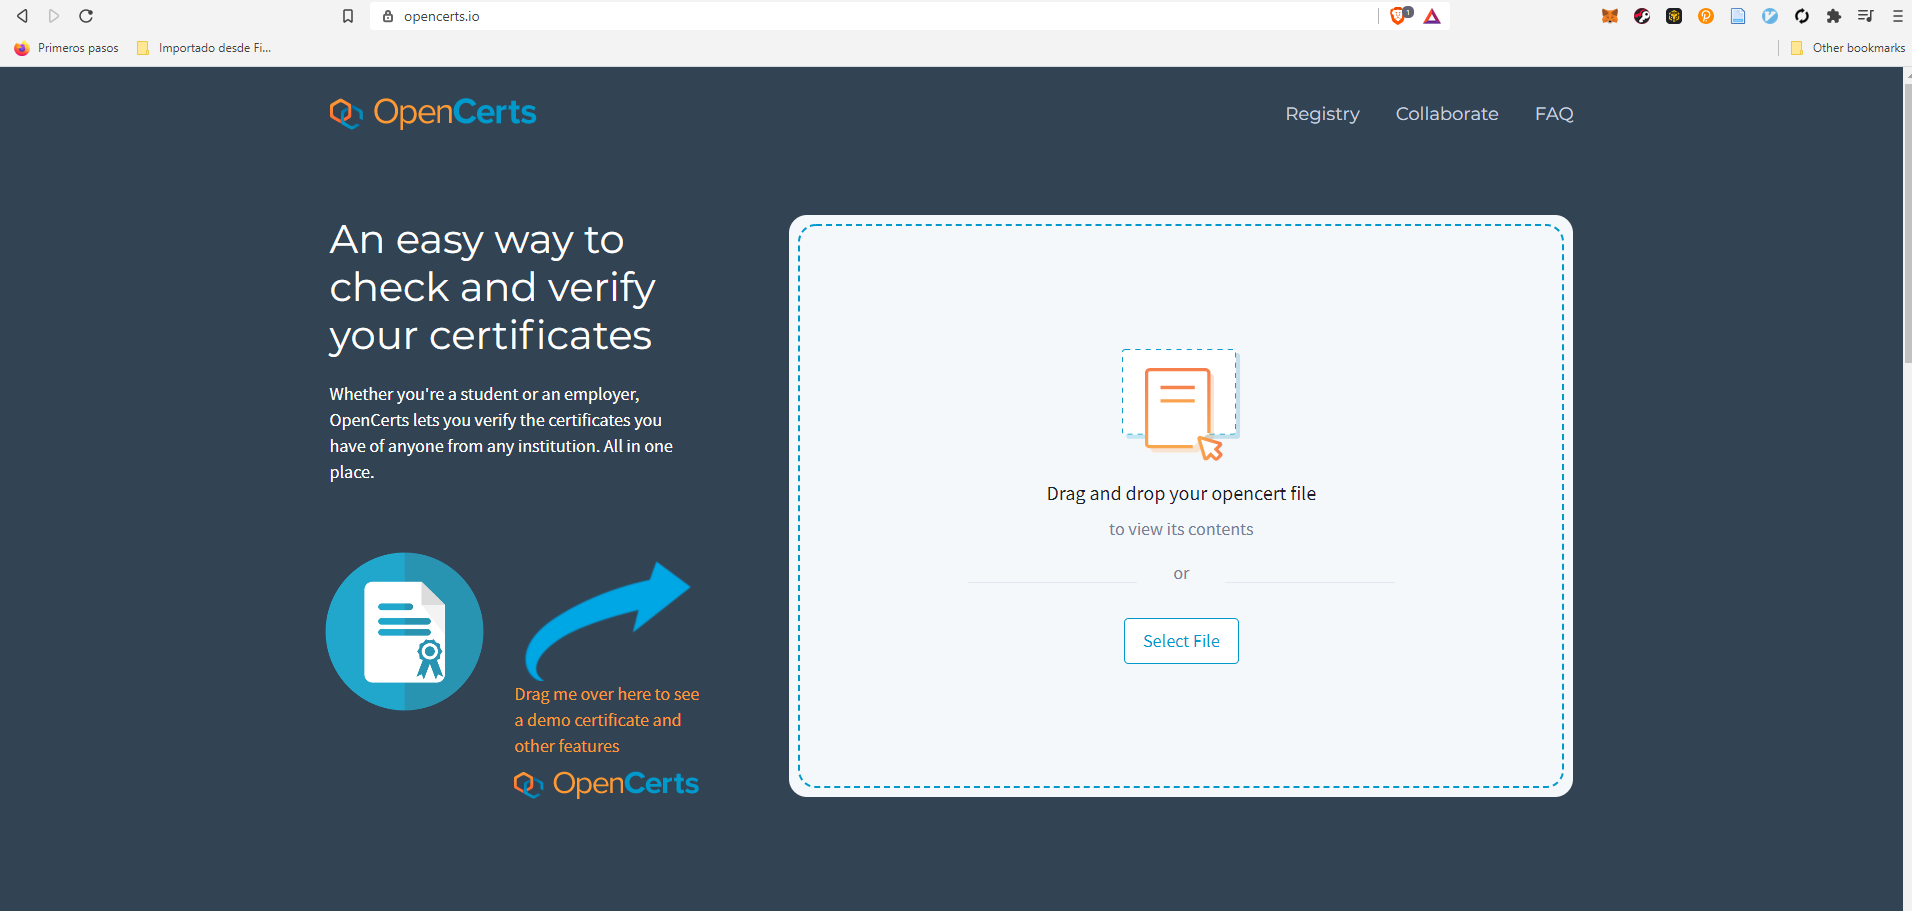
\includegraphics[scale=0.3]{OpenCerts_Home.png}}
  \caption{Página Web de OpenCerts}
  \label{img:opencerts_home}
\end{figure}

En la imagen \ref{img:opencerts_home} se puede observar lo sencillo que es verificar un documento. Simplemente se arrastra el  archivo 
de extensión“.opencerts”
y se buscará en la  Blockchain si realmente fue emitido por alguna entidad.
OpenCerts utiliza los smart contract en la  Blockchain de Ethereum. También utiliza tecnologías como Ract.js, Metamask, Web3.js, entre otros. 
Lo que permite desarrollar
un sistema de certificados totalmente descentralizado \cite[]{opencerts_gestion_nodate}. 